\documentclass{article}
\usepackage{amsmath}
\usepackage{amssymb}
\usepackage{graphicx}
\usepackage{tikz}
\usepackage{tikz-feynman}
\usetikzlibrary{shapes,arrows,positioning}
\usepackage{caption} % 添加此行以支持\captionof

\begin{document}

\section*{I.7.2}

We want to find the mathematical expression for the s-channel one-loop diagram in $\phi^4$ theory.

\begin{center}
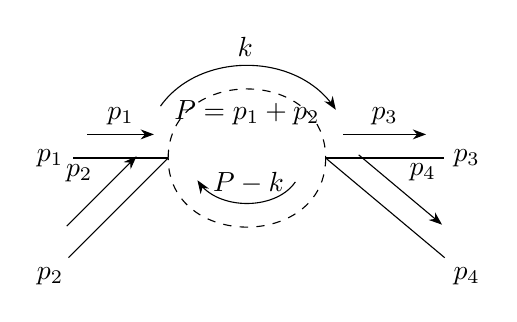
\begin{tikzpicture}
\begin{feynman}
    % Define vertices
    \vertex (i1) {\(p_1\)}; % Incoming particle 1
    \vertex [right=of i1] (v1); % First interaction vertex
    \vertex [right=2cm of v1] (v2); % Second interaction vertex (2cm to the right of v1)
    \vertex [right=of v2] (o1) {\(p_3\)}; % Outgoing particle 1

    \vertex [below=of i1] (i2) {\(p_2\)}; % Incoming particle 2
    \vertex [below=of o1] (o2) {\(p_4\)}; % Outgoing particle 2

    % Draw external lines
    \diagram* {
        (i1) -- [momentum=\(p_1\)] (v1),
        (i2) -- [momentum=\(p_2\)] (v1),
        (v2) -- [momentum=\(p_3\)] (o1),
        (v2) -- [momentum=\(p_4\)] (o2),
    };

    % Draw loop lines between v1 and v2
    \diagram* {
        (v1) -- [scalar, half left, looseness=1.5, momentum=\(k\)] (v2), % First loop propagator
        (v2) -- [scalar, half left, looseness=1.5, momentum'=\(P-k\)] (v1), % Second loop propagator, where P = p1+p2
    };

    % Add label for total incoming momentum P = p1 + p2
    \node [above=0.3cm of $(v1)!0.5!(v2)$] {\(P = p_1+p_2\)};

\end{feynman}
\end{tikzpicture}
\captionof{figure}{The s-channel one-loop Feynman diagram.}
\end{center}

The final expression for the invariant amplitude, $i\mathcal{M}_s$, is:
$$i\mathcal{M}_s = \frac{1}{2}(-i\lambda)^2 \int \frac{d^4 k}{(2\pi)^4} \frac{i}{k^2 - m^2 + i\epsilon} \frac{i}{(k_1 + k_2 - k)^2 - m^2 + i\epsilon}$$
The key is to derive the coefficient, especially the \textbf{symmetry factor} of $1/2$.


\section*{Origin and Calculation}

This diagram arises from the second-order term in the perturbative expansion of Formula B:
$$\frac{1}{2!} \left( -i \int d^4y \frac{\lambda}{4!}\phi^4(y) \right)^2$$
The coefficient is found by counting the number of ways to perform the Wick contractions that form the diagram's topology.

\begin{center}
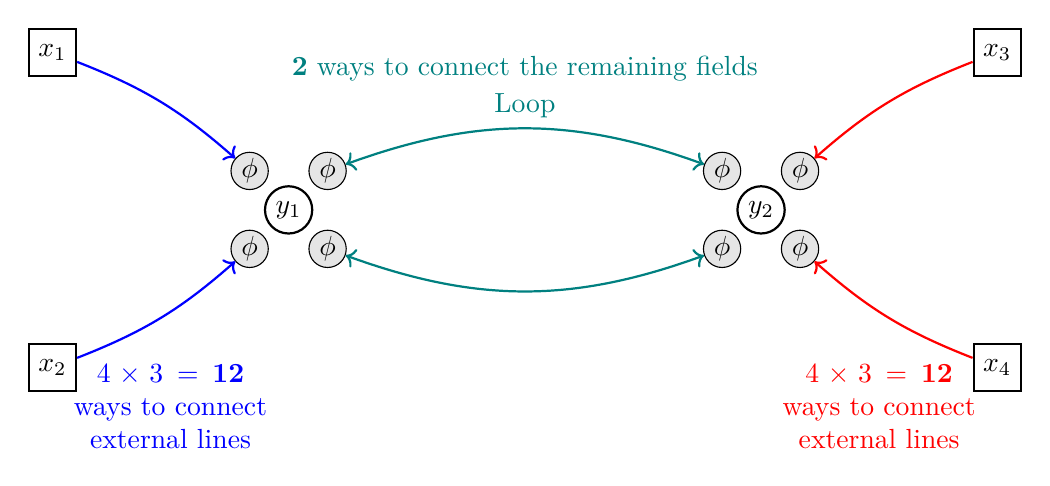
\begin{tikzpicture}[
    vtx/.style={circle, draw, thick, inner sep=2pt, minimum size=6mm},
    ext/.style={rectangle, draw, thick, inner sep=2pt, minimum size=6mm},
    phi/.style={circle, draw, fill=gray!20, inner sep=1pt, minimum size=3mm}
]
% Vertex 1
\node[vtx] (V1) at (0,0) {\(y_1\)};
\foreach \i/\pos in {1/135, 2/45, 3/225, 4/315} {
    \node[phi] (p1\i) at ([shift=(\pos:0.7cm)]V1) {\(\phi\)};
}

% Vertex 2
\node[vtx] (V2) at (6,0) {\(y_2\)};
\foreach \i/\pos in {1/135, 2/45, 3/225, 4/315} {
    \node[phi] (p2\i) at ([shift=(\pos:0.7cm)]V2) {\(\phi\)};
}

% External Legs
\node[ext] (x1) at (-3, 2) {\(x_1\)};
\node[ext] (x2) at (-3,-2) {\(x_2\)};
\node[ext] (x3) at ( 9, 2) {\(x_3\)};
\node[ext] (x4) at ( 9,-2) {\(x_4\)};

% Contractions
\draw[->, thick, blue] (x1) to[bend left=10] (p11);
\draw[->, thick, blue] (x2) to[bend right=10] (p13);
\draw[->, thick, red] (x3) to[bend right=10] (p22);
\draw[->, thick, red] (x4) to[bend left=10] (p24);
\draw[<->, thick, teal] (p12) to[bend left=20] node[midway, above] {Loop} (p21);
\draw[<->, thick, teal] (p14) to[bend right=20] node[midway, below] {} (p23);

% Annotations
\node[blue, text width=3cm, align=center] at (-1.5, -2.5) {$4 \times 3 = \mathbf{12}$ ways to connect external lines};
\node[red, text width=3cm, align=center] at (7.5, -2.5) {$4 \times 3 = \mathbf{12}$ ways to connect external lines};
\node[teal] at (3, 1.8) {$\mathbf{2}$ ways to connect the remaining fields};

\end{tikzpicture}
\captionof{figure}{Visualizing the Wick contractions and counting the combinations.}
\end{center}

Let's count the connections:
\begin{enumerate}
    \item \textbf{Connect external lines to vertex $y_1$}: There are $4 \times 3 = \mathbf{12}$ ways.
    \item \textbf{Connect external lines to vertex $y_2$}: There are $4 \times 3 = \mathbf{12}$ ways.
    \item \textbf{Form the loop}: Two fields remain at each vertex. There are $\mathbf{2}$ ways to connect them.
\end{enumerate}

Now, we combine this with the factors from the Lagrangian.
\begin{align*}
    \text{Coefficient} &= \underbrace{\left(\frac{-i\lambda}{4!}\right)^2}_{\text{Vertex Factors}} \times \underbrace{(12 \times 12 \times 2)}_{\text{Contractions}} \\
    &= \frac{(-i\lambda)^2}{(24)^2} \times 288 \\
    &= \frac{(-i\lambda)^2}{576} \times 288 \\
    &= \frac{1}{2}(-i\lambda)^2
\end{align*}
This calculation correctly produces the \textbf{symmetry factor of 1/2}.

\end{document}